\documentclass[11pt]{article}
\usepackage[utf8]{inputenc}
\usepackage[russian]{babel}
\usepackage[T1]{fontenc}
\usepackage{amssymb,amsmath,clrscode,graphicx,indentfirst}

\author{Олег Смирнов}
\title{Курс kiev-clrs -- Лекция 17. Кратчайшие пути: алгоритм Дейкстры, поиск в ширину}
\date{11 июля 2009 г.}

\begin{document}
\maketitle
\tableofcontents
\newpage
\setlength{\parskip}{1ex plus 0.5ex minus 0.2ex}
\section{Цель лекции}
\begin{itemize}
\item Задача кратчайшего пути в нагруженном графе
\item Поиск в ширину
\end{itemize}

\section{Задача кратчайшего пути}
Задач поиска кратчайшего (минимального) пути в графе является приложением динамического программирования и жадных алгоритмов.

В ориентированном графе $G = (V,E)$ с весами дуг заданными как $w~:~E~\to~\mathbb{R}$, направленный путь $p = v_1 \to v_2 \to \ldots \to v_k$ имеет вес
\begin{equation*}
  w(p) = \sum_{i=1}^{k-1}w(v_i, v_{i+1})
\end{equation*}
\begin{figure}[h!]
  \centering
  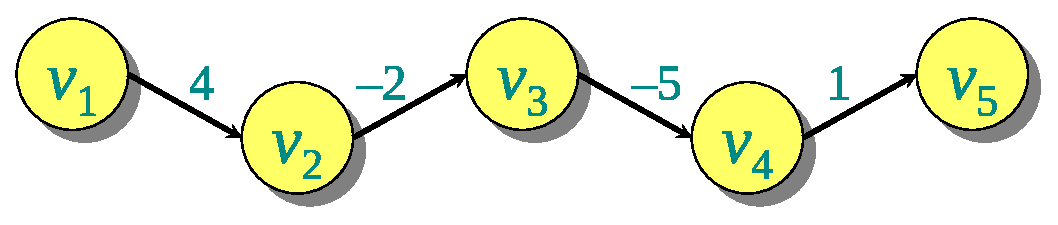
\includegraphics[width=3in]{lecture17/path1.eps}
  \caption{Путь с весом $w(p) = -2$}
\end{figure}

\textbf{Крачайший путь} из $u$ в $v$ -- это путь с минимальным возможным весом из $u$ в $v$:
\begin{equation*}
  \delta(u, v) = \min\{w(p):\text{ из }u\text{ в }v\}
\end{equation*}

Кратчайшие пути могут не существовать, когда в графе есть дуги с отрицательным весом. В этом случае $\delta(u, v) = -\infty$.
\begin{figure}[h!]
  \centering
  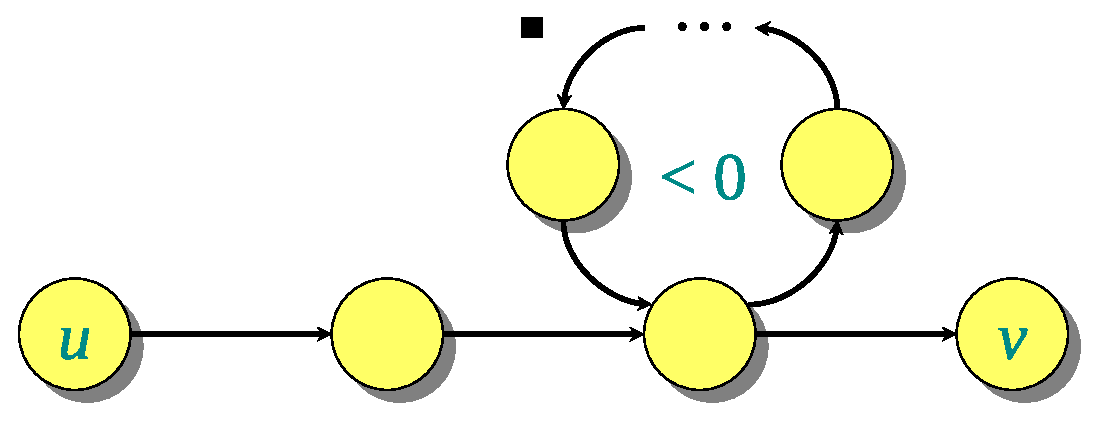
\includegraphics[width=3in]{lecture17/path2.eps}
  \caption{Отрицательный путь}
\end{figure}

Отрицательный цикл в графе можно обходить бесконечное количество раз, уменьшая вес пути.

Кратчайшие пути могут не существовать, если граф несвязный. В этом случае, если путь из $u$ в $v$ отсутствует, обозначают $\delta(u, v) = \infty$.

Для реализации алгоритма поиска кратчайших путей нужно доказать две леммы о свойствах кратчайших путей.
\begin{enumerate}
\item Свойство оптимальной подструктуры: подпуть кратчайшего пути тоже является кратчайшим путём.
\begin{figure}[h!]
  \centering
  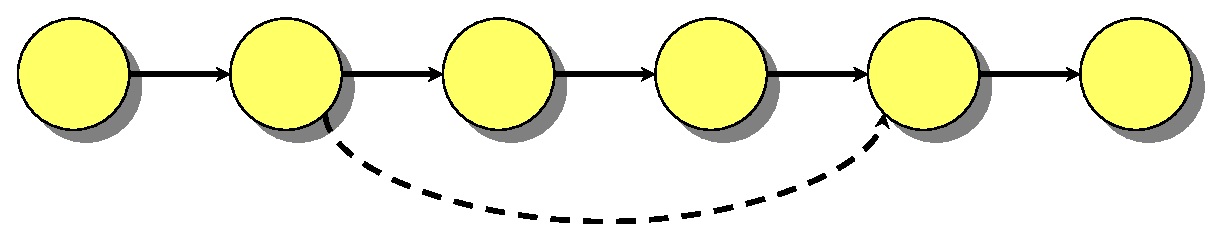
\includegraphics[width=3in]{lecture17/cutpaste.eps}
  \caption{Оптимальная подструктура}
\end{figure}

Допустим существует подпуть, которые короче рассматриваемого. Тогда удалив из исходного пути рассматриваемый и добавив более короткий, мы получим путь, который оптимальный исходного. Это противоречие доказывает лемму.
\item Неравенство треугольника: для всех вершин $u, v, x \in V$ выполняется неравенство
\begin{equation*}
  \delta(u, v) \leqslant \delta(u, x) + \delta(x, v)
\end{equation*}
\begin{figure}[h!]
  \centering
  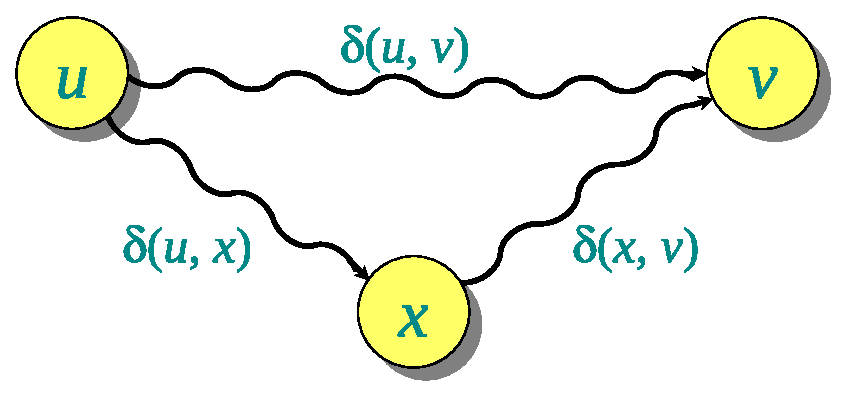
\includegraphics[width=2in]{lecture17/triangle.eps}
  \caption{Неравенство треугольника}
\end{figure}
Можно увидеть, что по определению, $\delta(u, v)$ является кратчайшим из всех возможных путей из $u$ в $v$, а значит он короче и пути из $u$ в $v$ через $x$ (сумма в правой части неравнства).
\end{enumerate}

\section{Кратчайшие пути из одной вершины}
Задача: найти длины всех кратчайших путей из заданной вершины $s \in V$ (исток) во все вершины $\delta(s, v)$ для $v \in V$.

\textbf{Известно, что задача поиска кратчайшего пути между двумя вершинами такая же по сложности, как задача поиска из одной вершины во все.}

Для упрощения задачи допустим, что в графе отсутствуют дуги отрицательного веса: $w(u, v) \geqslant 0$, $\forall u, v \in V$. Это означает, что кратчайшие пути существуют и $\delta(u, v) > - \infty$.

Идея: использовать жадный алгоритм.
\begin{itemize}
\item на каждом шаге поддерживается инвариант -- множество $S$ вершин, для которых уже известны длины кратчайших путей из истока $s$ (в начале $s \in S$)
\item на каждом шаге в множество $S$ добавляется вершина $v \in V-S$, для которой оценка дистанции из $s$ минимальна
\item после этого происходит обновление (релаксация) оценок путей для вершин, смежных с $v$
\end{itemize}
Идея алгоритма в том, что из исходного графа выделяется подмножество вершин, кратчайшие расстояния к которым до $s$ мы уже знаем. В отдельной структуре хранятся оценки расстояния от этого облака к остальному графу. Если оценка неизвестна, то она принимается равной $\infty$. На каждом шаге алгоритм выбирает из графа ту вершину, которая ``ближе'' (оценка расстояния минимальна) -- это ``жадный'' выбор. После того, как эта вершина добавляется к множеству известных, оценки расстояний до других вершин корректируются (релаксируются).
\section{Алгоритм Дейкстры}
\begin{codebox}
\Procname{$\proc{Shortest\_Paths}(V)$}
\li $d[s] \gets 0$
\li \For each $v \in V - \{s\}$
\li     \Do $d[v] \gets \infty$ \Comment $d[x]$ -- оценка пути из $s$ в $x$ \\
\Comment $d[x]$ будет равно дистанции $\delta(s, x)$ если $x \in S$
    \End
\li $S \gets \emptyset$
\li $Q \gets V$ \Comment $Q$ -- очередь с приоритетом для $V-S$, \\
\Comment где ключём является $d[v]$. В начале содержит все вершины
\li \While $Q \neq \emptyset$
\li     \Do $u \gets Extract\_Min(Q)$
\li         $S \gets S \cup \{u\}$
\li         \For each $v \in Adj[u]$
\li             \Do \If $d[v] > d[u] + w(u, v)$ \Comment шаг релаксации
\li                 \Then $d[v] \gets d[u] + w(u, v)$
                    \End
            \End
    \End
\li \Return $d$
\end{codebox}
Для доказательства корректности нужно показать, что шаг релаксации находит все кратчайшие пути в графе. Его условие является неравенством треугольника, доказанным выше. Внутри шага релаксации при уменьшении значения ключа $d[v]$ происходит реорганизация очереди с приоритетом.

Первый шаг -- инициализация алгоритма: $S = \{\}$
\begin{figure}[h!]
  \centering
  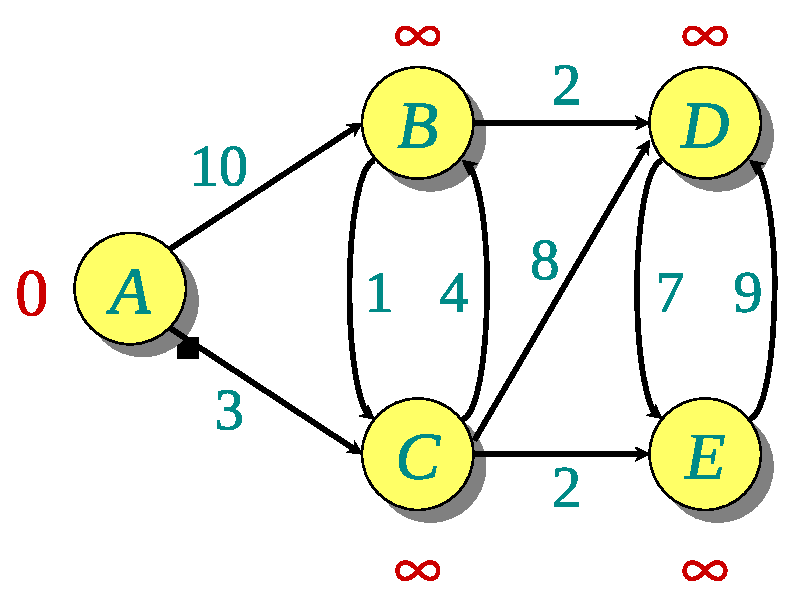
\includegraphics[width=2in]{lecture17/dijkstra1.eps}
  \caption{Шаг 1}
\end{figure}
\begin{center}
\begin{tabular}{|r|c|c|c|c|c|}
  \hline
     $Q$ & \textbf{A} & \textbf{B} & \textbf{C} & \textbf{D} & \textbf{E} \\
  \hline
         & 0 & $\infty$ & $\infty$ & $\infty$ & $\infty$  \\
  \hline
\end{tabular}
\end{center}
\newpage
На втором шаге: $A \leftarrow Extract\_Min(Q)$.
\begin{figure}[h!]
  \centering
  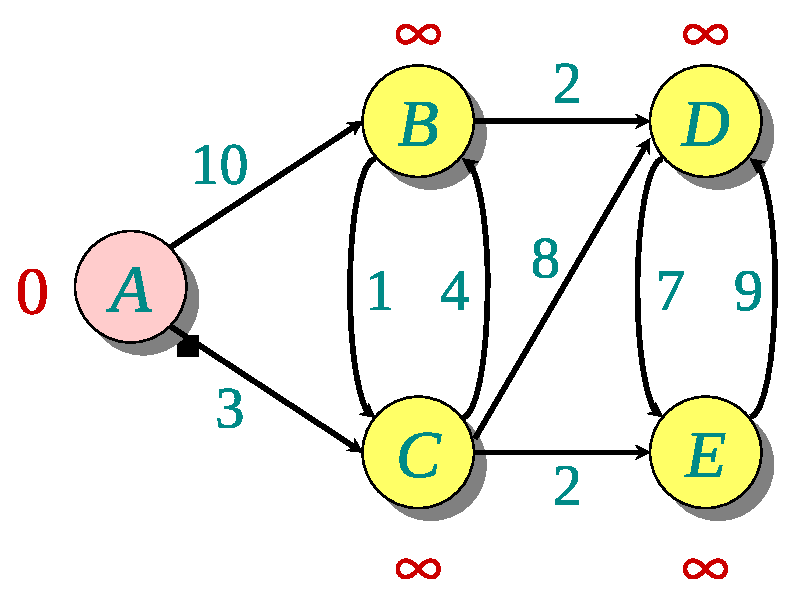
\includegraphics[width=2in]{lecture17/dijkstra2.eps}
  \caption{Шаг 2}
\end{figure}
\begin{center}
\begin{tabular}{|r|c|c|c|c|c|}
  \hline
     $Q$ & A & \textbf{B} & \textbf{C} & \textbf{D} & \textbf{E} \\
  \hline
         & \textbf{0} & $\infty$ & $\infty$ & $\infty$ & $\infty$ \\
  \hline
\end{tabular}
\end{center}
\begin{equation*}
  S = \{A\}
\end{equation*}
Релаксация дуг, смежных с $A$:
\begin{figure}[h!]
  \centering
  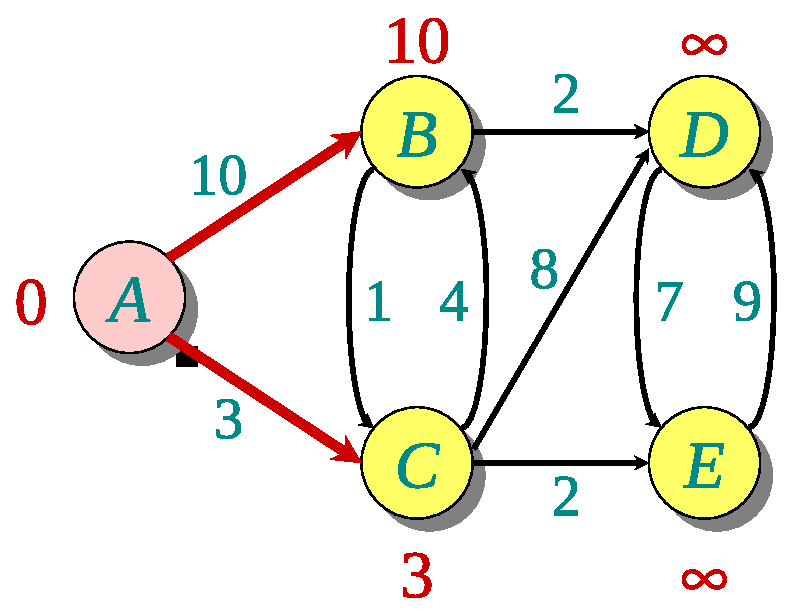
\includegraphics[width=2in]{lecture17/dijkstra21.eps}
  \caption{Шаг 2.1}
\end{figure}
\begin{center}
\begin{tabular}{|r|c|c|c|c|c|}
  \hline
     $Q$ & A & \textbf{B} & \textbf{C} & \textbf{D} & \textbf{E} \\
  \hline
         & \textbf{0} & $\infty$ & $\infty$ & $\infty$ & $\infty$ \\
  \hline
         & & 10 & 3 & $\infty$ & $\infty$ \\
  \hline
\end{tabular}
\end{center}
\newpage
Шаг три: минимальный приоритет в очереди имеет элемент $C \leftarrow Extract\_Min(Q)$.
\begin{figure}[h!]
  \centering
  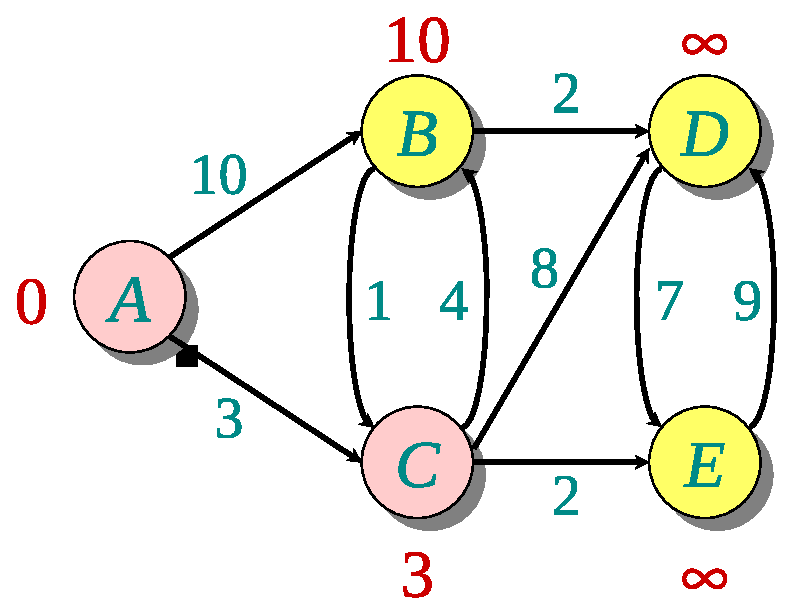
\includegraphics[width=2in]{lecture17/dijkstra3.eps}
  \caption{Шаг 3}
\end{figure}
\begin{center}
\begin{tabular}{|r|c|c|c|c|c|}
  \hline
     $Q$ & A & \textbf{B} & C & \textbf{D} & \textbf{E} \\
  \hline
         & \textbf{0} & $\infty$ & $\infty$ & $\infty$ & $\infty$ \\
  \hline
         & & 10 & \textbf{3} & $\infty$ & $\infty$ \\
  \hline
\end{tabular}
\end{center}
\begin{equation*}
  S = \{A, C\}
\end{equation*}
Релаксация дуг, смежных с $C$:
\begin{figure}[h!]
  \centering
  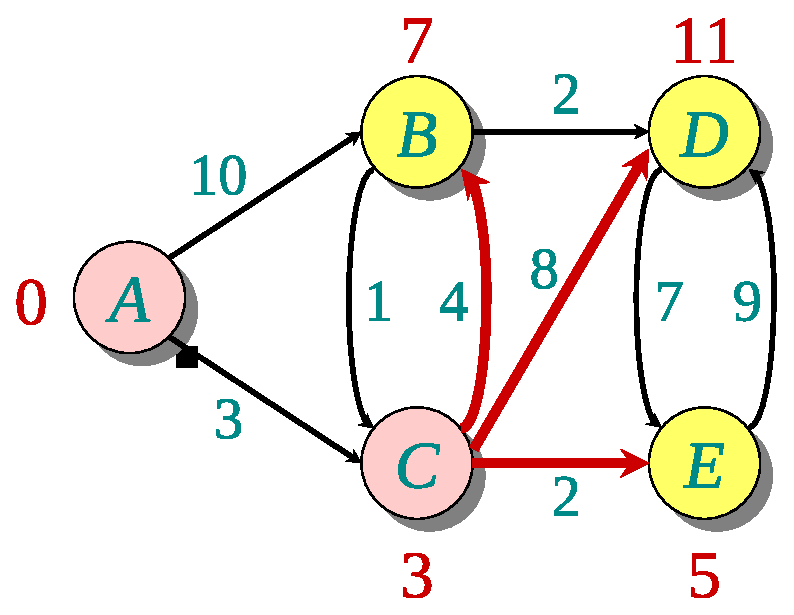
\includegraphics[width=2in]{lecture17/dijkstra31.eps}
  \caption{Шаг 3.1}
\end{figure}
\begin{center}
\begin{tabular}{|r|c|c|c|c|c|}
  \hline
     $Q$ & A & \textbf{B} & C & \textbf{D} & \textbf{E} \\
  \hline
         & \textbf{0} & $\infty$ & $\infty$ & $\infty$ & $\infty$ \\
  \hline
         & & 10 & \textbf{3} & $\infty$ & $\infty$ \\
  \hline
         & & 7 & & 11 & 5 \\
  \hline
\end{tabular}
\end{center}
\newpage
Шаг четыре: $E \leftarrow Extract\_Min(Q)$
\begin{figure}[h!]
  \centering
  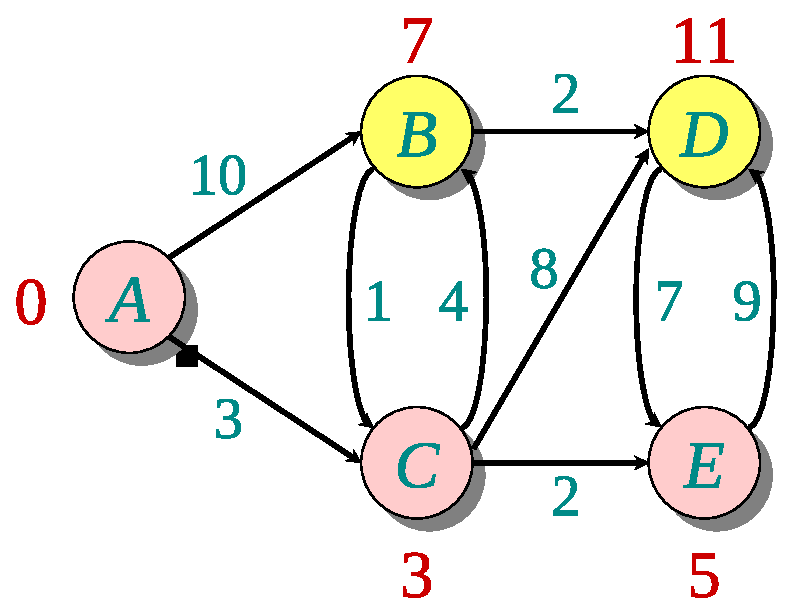
\includegraphics[width=2in]{lecture17/dijkstra4.eps}
  \caption{Шаг 4}
\end{figure}
\begin{center}
\begin{tabular}{|r|c|c|c|c|c|}
  \hline
     $Q$ & A & \textbf{B} & C & \textbf{D} & E \\
  \hline
         & \textbf{0} & $\infty$ & $\infty$ & $\infty$ & $\infty$ \\
  \hline
         & & 10 & \textbf{3} & $\infty$ & $\infty$ \\
  \hline
         & & 7 & & 11 & \textbf{5} \\
  \hline
\end{tabular}
\end{center}
\begin{equation*}
  S = \{A, C, E\}
\end{equation*}
Релаксация дуг, смежных с $E$:
\begin{figure}[h!]
  \centering
  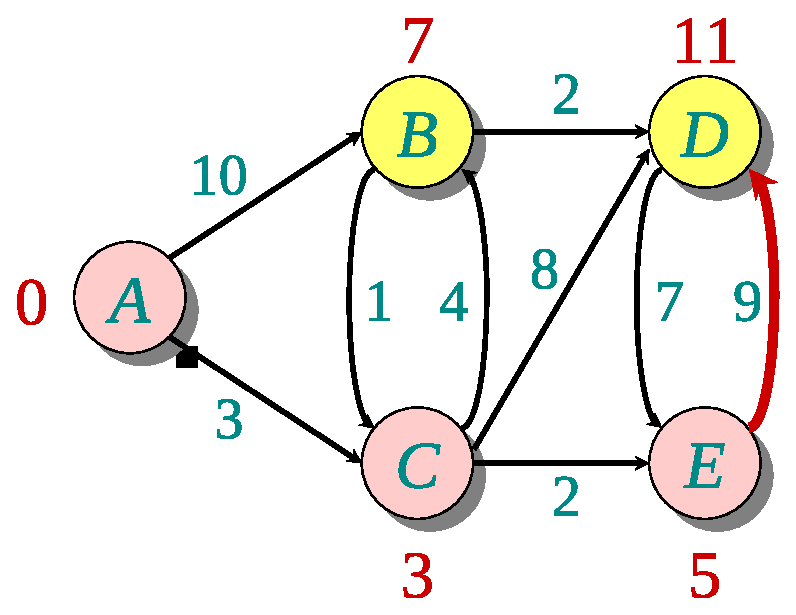
\includegraphics[width=2in]{lecture17/dijkstra41.eps}
  \caption{Шаг 4.1}
\end{figure}
\begin{center}
\begin{tabular}{|r|c|c|c|c|c|}
  \hline
     $Q$ & A & \textbf{B} & C & \textbf{D} & E \\
  \hline
         & \textbf{0} & $\infty$ & $\infty$ & $\infty$ & $\infty$ \\
  \hline
         & & 10 & \textbf{3} & $\infty$ & $\infty$ \\
  \hline
         & & 7 & & 11 & \textbf{5} \\
  \hline
         & & 7 & & 11 & \\
  \hline
\end{tabular}
\end{center}
\newpage
$B \leftarrow Extract\_Min(Q)$.
\begin{figure}[h!]
  \centering
  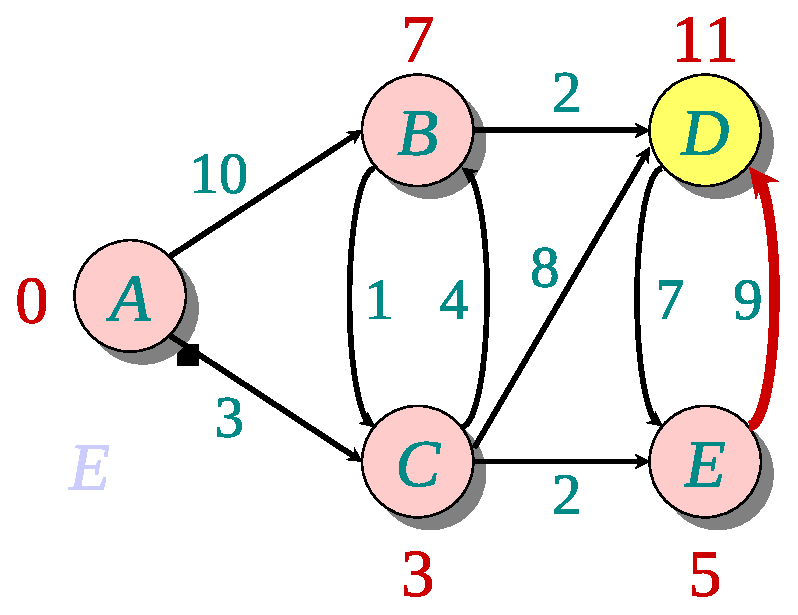
\includegraphics[width=2in]{lecture17/dijkstra5.eps}
  \caption{Шаг 5}
\end{figure}
\begin{center}
\begin{tabular}{|r|c|c|c|c|c|}
  \hline
     $Q$ & A & B & C & \textbf{D} & E \\
  \hline
         & \textbf{0} & $\infty$ & $\infty$ & $\infty$ & $\infty$ \\
  \hline
         & & 10 & \textbf{3} & $\infty$ & $\infty$ \\
  \hline
         & & 7 & & 11 & \textbf{5} \\
  \hline
         & & \textbf{7} & & 11 & \\
  \hline
\end{tabular}
\end{center}
\begin{equation*}
  S = \{A, C, E, B\}
\end{equation*}
Релаксация дуг, смежных с $B$:
\begin{figure}[h!]
  \centering
  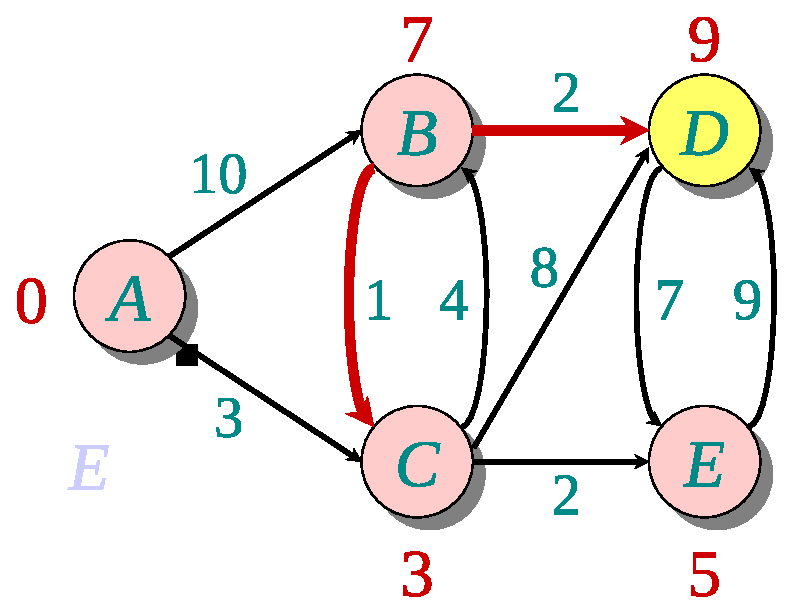
\includegraphics[width=2in]{lecture17/dijkstra51.eps}
  \caption{Шаг 5.1}
\end{figure}
\begin{center}
\begin{tabular}{|r|c|c|c|c|c|}
  \hline
     $Q$ & A & B & C & \textbf{D} & E \\
  \hline
         & \textbf{0} & $\infty$ & $\infty$ & $\infty$ & $\infty$ \\
  \hline
         & & 10 & \textbf{3} & $\infty$ & $\infty$ \\
  \hline
         & & 7 & & 11 & \textbf{5} \\
  \hline
         & & \textbf{7} & & 11 & \\
  \hline
         & & & & 9 & \\
  \hline
\end{tabular}
\end{center}
\newpage
$D \leftarrow Extract\_Min(Q)$.
\begin{figure}[h!]
  \centering
  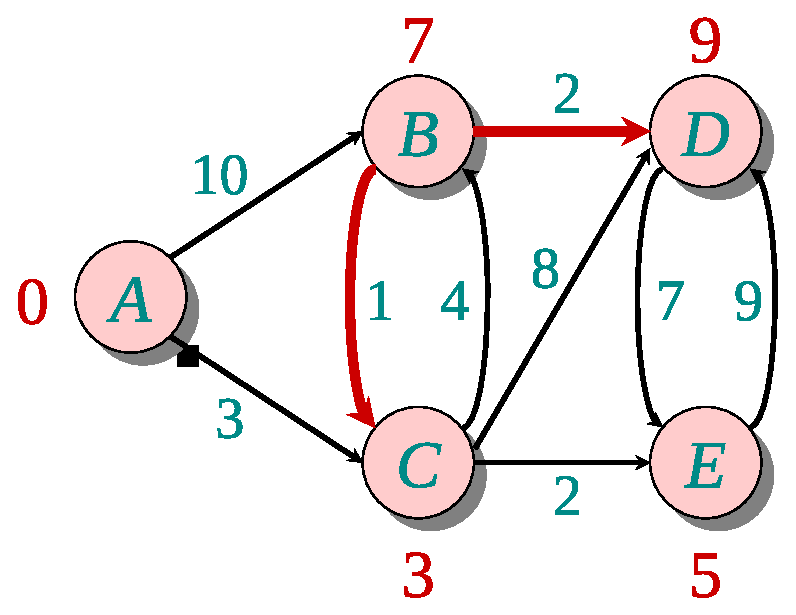
\includegraphics[width=2in]{lecture17/dijkstra6.eps}
  \caption{Шаг 6}
\end{figure}
\begin{center}
\begin{tabular}{|r|c|c|c|c|c|}
  \hline
     $Q$ & A & B & C & D & E \\
  \hline
         & \textbf{0} & $\infty$ & $\infty$ & $\infty$ & $\infty$ \\
  \hline
         & & 10 & \textbf{3} & $\infty$ & $\infty$ \\
  \hline
         & & 7 & & 11 & \textbf{5} \\
  \hline
         & & \textbf{7} & & 11 & \\
  \hline
         & & & & \textbf{9} & \\
  \hline
\end{tabular}
\end{center}
\begin{equation*}
  S = \{A, C, E, B, D\}
\end{equation*}
Если алгоритм корректен,то  длины путей, содержащиеся в массиве $d$ -- минимально возможные в данном графе.

Для того, чтоб найти минимальные пути в графе, нужно рассмотреть для каждой вершины $v$ последнюю дугу$(u, v)$, которая подвергалась релаксации. Совокупность таких дуг образует дерево с вершиной в $s$ и уникальными путями вниз до каждой из вершины $v$. Каждый путь в дереве соответствует минимальному в графе.
\section{Корректность алгоритма}
Корректность алгоритма доказывается по частям.
\begin{enumerate}
\item Отсутствие ошибок в цикле релаксации: $d[v]$ всегда служит верхней оценкой $\delta(s, v)$, т.е. инвариант $d[v] \geqslant \delta(s, v)$ выполняется для всех $v \in V$ на каждом из шагов после инициализации.

Доказательство по индукции.
\begin{itemize}
\item Базовый случай: $d[s] \leftarrow 0$ и $d[v] \leftarrow \infty$, $\forall v \neq s$
  выполняется, т.к. $\delta(s, s) = 0$ и $\delta(s, v) \leqslant \infty$
\item Предположим, что инвариант не выполняется на одном из шагов. Пусть $d[v] < \delta(s, v)$ было получено на шаге релаксации $d[v] \leftarrow d[u] + w(u, v)$. Тогда:
  \begin{align*}
    d[u] + w(u, v) \geqslant \\
    \delta(s, u) + w(u, v) \geqslant \\
    \delta(s, u) + \delta(u, v) \geqslant \\
    \geqslant \delta(s, v)
  \end{align*}
Противоречие доказывает лемму. Идея в том, что каждое присваивание на шаге релаксации оперирует с реальным путем в графе, а длина каждого пути всегда больше или равна длине кратчайшего пути.
\end{itemize}
\item Кратчайшие пути: пусть $s \to \ldots \to u \to v$ -- кратчайший путь из $s$ в $v$ и пусть $d[u] = \delta(s, u)$. Тогда после шага релаксации дуги $(u, v)$ выполнится $d[v] = \delta(s, v)$.

По первой лемме, $d[v] \geqslant \delta(s, v)$. Если $d[v] > \delta(s, v)$, то выполнится условие релаксации и тогда $d[v] \leftarrow d[u] + w(u, v)$, т.е. $d[v] = \delta(s, v)$.
\item Завершение алгоритма: когда алгоритм Дейкстры заканчивает работу, $d[v] = \delta(s, v)$ для всех $v \in V$.

Легко увидеть, что $d[v]$ не изменяется после того, как $v \in S$. Допустим, что перед добавлением $u$ в $S$: $d[u] \neq \delta(s, u)$. Следовательно, по первой лемме $d[u] > \delta(s, u)$.

Пусть $p$ -- кратчайший путь из $s$ в $u$. Т.е. $w(p) = \delta(s, u)$. Рассмотрим первую дугу $(x, y)$, в которой путь $p$ выходит за пределы $S$.
\begin{align*}
  \text{Т.к. }x \in S: \\
  d[x] = \delta(s, x) \\
  \text{При релаксации по первой лемме:} \\
  d[y] = \delta(s, y) \leqslant \\
  \text{Т.к. путь до }y\text{ является подпутем до }u\text{ :} \\
  \leqslant \delta(s, u) \\
  \text{Но по правилу выбора из очереди:} \\
  d[u] \leqslant d[y]
\end{align*}
\begin{figure}[h!]
  \centering
  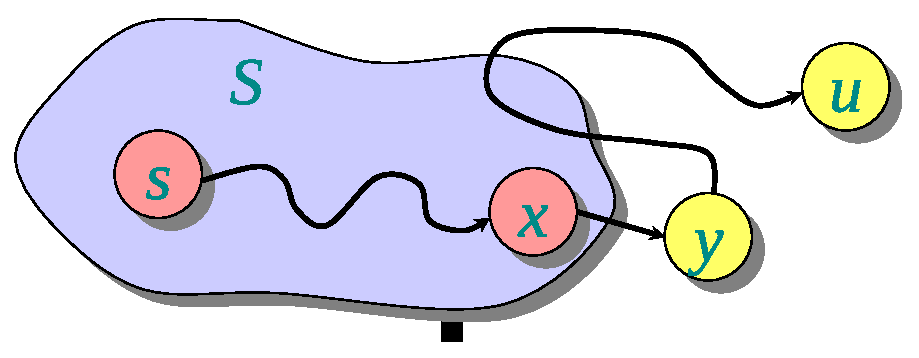
\includegraphics[width=2.5in]{lecture17/correctness.eps}
  \caption{Корректность завершения}
\end{figure}
\end{enumerate}

\section{Анализ алгоритма Дейкстры}
\begin{enumerate}
\item Время инициализации алгоритма линейно: $O(V)$
\item Цикл с $Extract\_Min$ выполняется для каждой вершины, время работы: $O(V)$
\item Цикл для смежных вершин выполнятеся за $O(degree(u))$ итераций
\item Согласно лемме о рукопожатиях, цикл выполнит $\Theta(E)$ релаксаций
\end{enumerate}
Время работы $T = \Theta(V) \cdot T_{Extract\_Min} + \Theta(E) \cdot T_{Decrease\_Key}$
\begin{center}
\begin{tabular}{|r|c|c|c|}
  \hline
     $Q$ & $T_{Extract\_Min}$ & $T_{Decrease\_Key}$ & Всего \\
  \hline
      массив & $O(V)$ & $O(1)$ & $O(V^2)$ \\
  \hline
      двоичная куча & $O(\lg V)$ & $O(\lg V)$ & $O(E \lg V)$ \\
  \hline
      Фиббоначева куча & $O(\lg V)$ & $O(1)$ & $O(E + V \lg V)$ \\
  \hline
\end{tabular}
\end{center}

\section{Поиск в ширину}
В ненагруженных графах, где можно считать что веса всех дуг $w(u, v) = 1$, алгоритм Дейкстры можно упросить, используя простую очередь (FIFO) вместо очереди с приоритетами.

Модификацией алгоритма для этого случая является поиск в ширину (Breadth-first search или BFS):
\begin{codebox}
\li \While $Q \neq \emptyset$
\li     \Do $u \gets Deq(Q)$
\li         \For each $v \in Adj[u]$
\li             \Do \If $d[v] = \infty$
\li                 \Then $d[v] \gets d[u] + 1$
\li                       $Enq(Q, v)$ \Comment $v$ в конец очереди
                    \End
            \End
    \End
\end{codebox}
На каждом шаге, если вершина еще не была посещена ($d[v] = \infty$), то кратчайший путь до неё равен пути до предшественника $u$ плюс единица. Затем $v$ добавляется в конец очереди.

В начале работы очередь $Q$ содержит только начальную вершину $s$.

Время работы алгоритма $T = O(V+E)$.

Инвариант алгоритма: на каждом шаге $v$ находится в очереди после $u$, откуда следует, что $d[v] = d[u]$ или $d[v] = d[u] +1$.
\end{document}
